\documentclass[12pt]{article}
\usepackage{fullpage,graphicx,psfrag,url,ar,rotating,float}
\usepackage[small,bf]{caption}
\usepackage{amsmath,amssymb,enumitem,bbm,subcaption,multirow}
\setlength{\captionmargin}{20pt}
\setlist[enumerate]{label=(\roman*)}

\title{\Large{AA274 (Winter 2017-18): Problem Set 2}}
\author{Anqi Fu}

\begin{document}
	\maketitle

\section{Camera Calibration}
\begin{enumerate}
	\item 
	\item 
	\item 
	\item 
	\item 
	\item 
\end{enumerate}

\section{Line Fitting}
\begin{enumerate}
	\item See submitted code.
	\item Using the suggested algorithm, I extracted the following lines for each data set.
	\begin{figure}[H]
		\centering
		\title{\bf Range Data $(x_r, y_r, n_{pts}) = (5,5,180)$ \\ \vspace{2.5mm}
			\verb|LINE_POINT_DIST_THRESHOLD = 0.05| \\
			\verb|MIN_POINTS_PER_SEGMENT = 0.065| \\
			\verb|MIN_SEG_LENGTH = 2| \\
			\verb|MAX_P2P_DIST = 0.8|}
		\\ \vspace{5mm}
		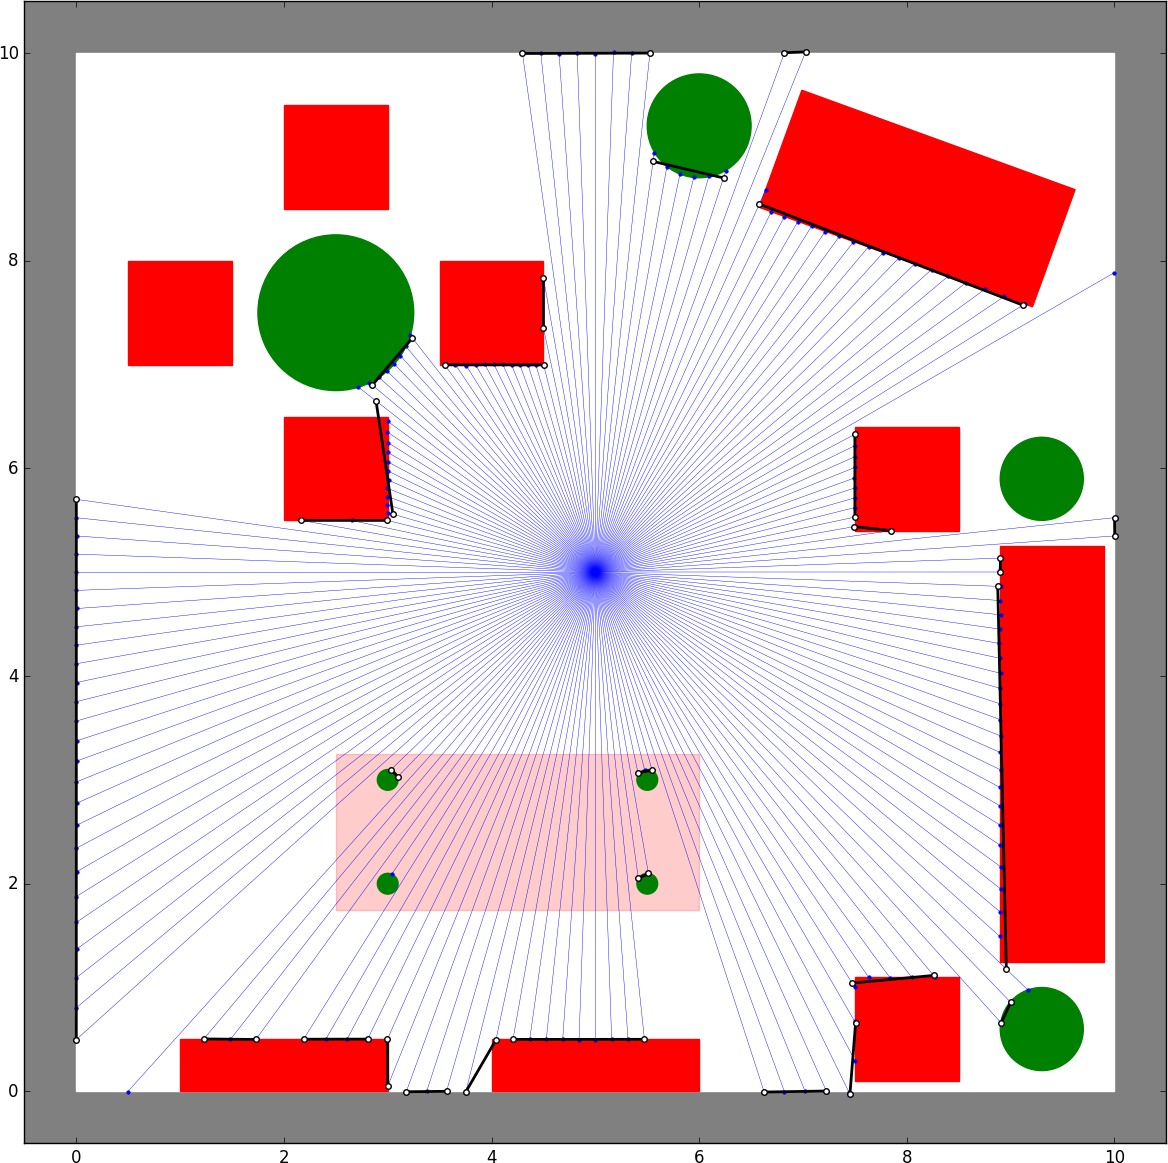
\includegraphics[width=0.8\textwidth]{../Figures/hw2_2_ii_55180.png}
	\end{figure}
	\begin{figure}[H]
		\centering
		\title{\bf Range Data $(x_r, y_r, n_{pts}) = (4,9,360)$ \\ \vspace{2.5mm}
			\verb|LINE_POINT_DIST_THRESHOLD = 0.05| \\
			\verb|MIN_POINTS_PER_SEGMENT = 0.025| \\
			\verb|MIN_SEG_LENGTH = 3| \\
			\verb|MAX_P2P_DIST = 0.54|}
		\\ \vspace{5mm}
		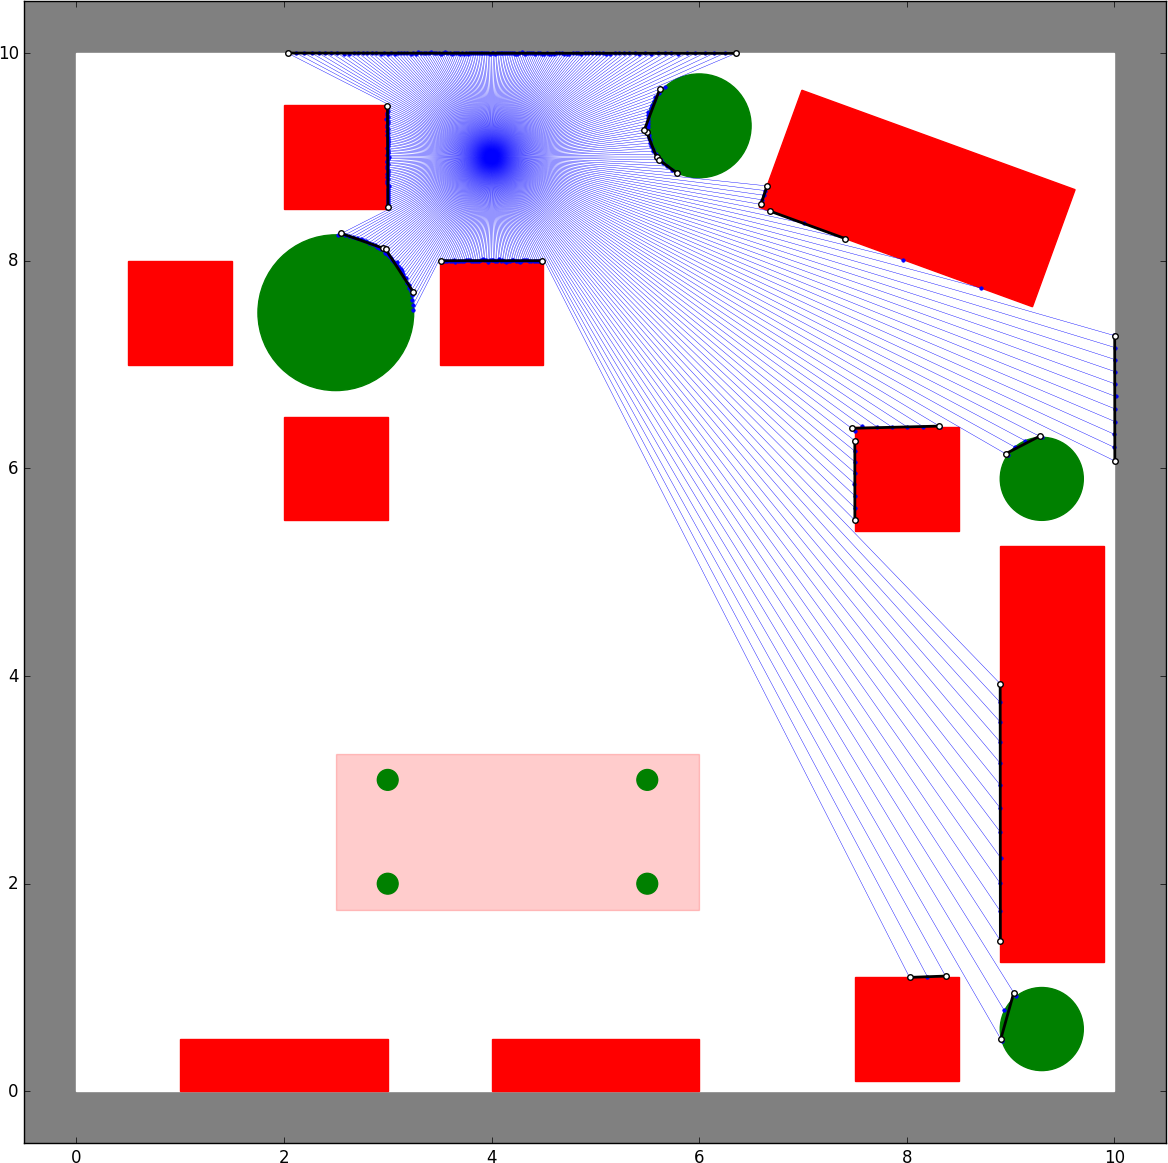
\includegraphics[width=0.8\textwidth]{../Figures/hw2_2_ii_49360.png}
	\end{figure}
	\begin{figure}[H]
		\centering
		\title{\bf Range Data $(x_r, y_r, n_{pts}) = (7,2,90)$ \\ \vspace{2.5mm}
			\verb|LINE_POINT_DIST_THRESHOLD = 0.05| \\
			\verb|MIN_POINTS_PER_SEGMENT = 0.165| \\
			\verb|MIN_SEG_LENGTH = 2| \\
			\verb|MAX_P2P_DIST = 0.42|}
		\\ \vspace{5mm}
		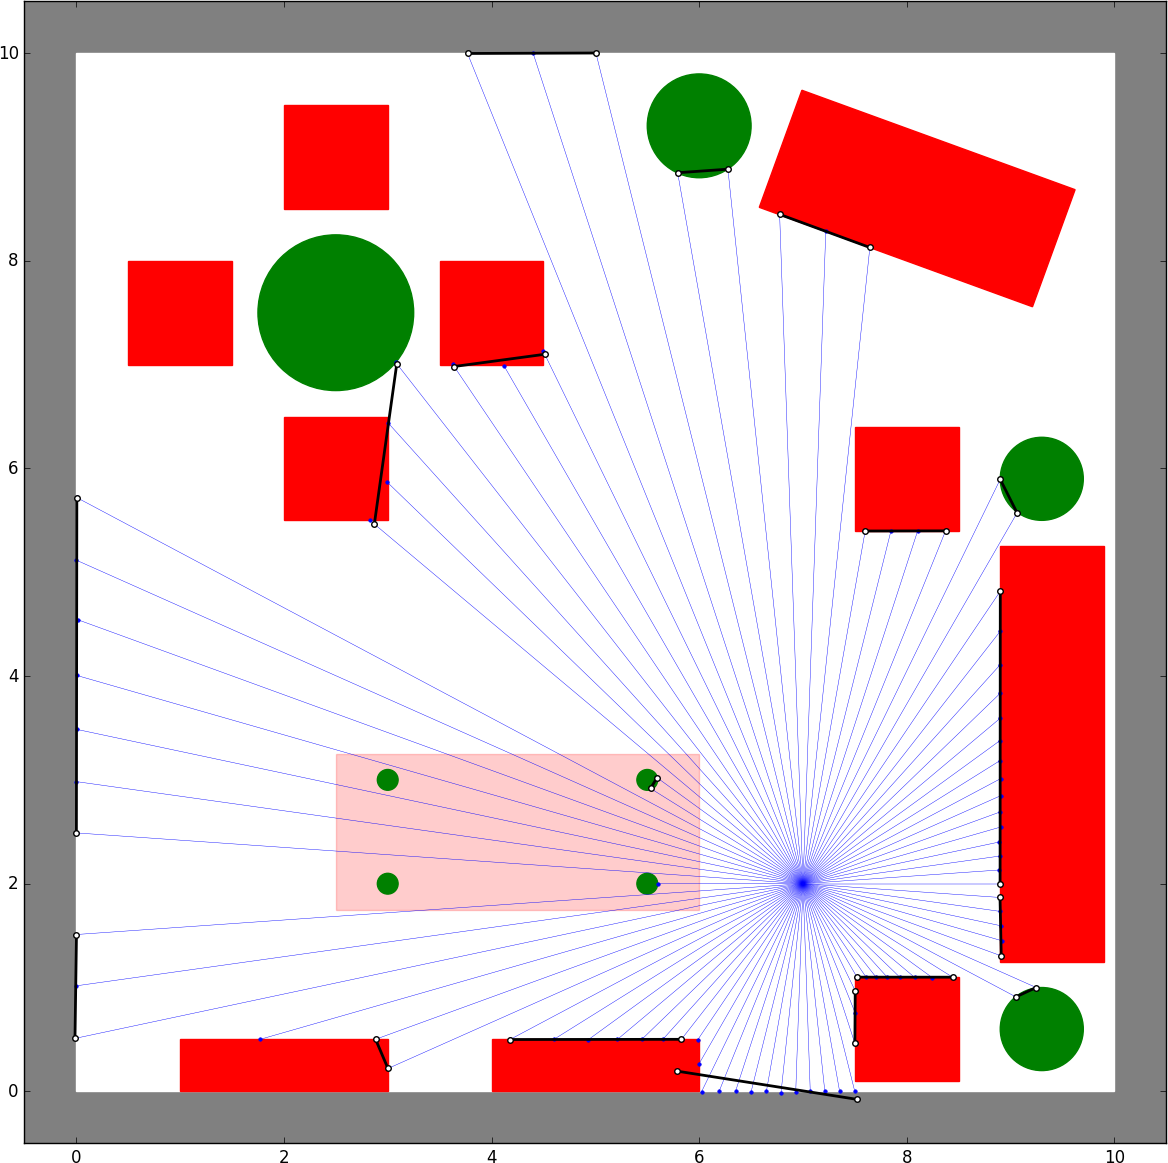
\includegraphics[width=0.8\textwidth]{../Figures/hw2_2_ii_7290.png}
	\end{figure}
\end{enumerate}

\end{document}